\documentclass{article}
\usepackage{tikz,tikzscale}
\usetikzlibrary{math}

\tikzset{pics/tpic/.style args={#1}{
    code={
      \draw (0,0) -- (5,5)
      node foreach \x in {1,...,#1} [circle,draw,pos=\x/(#1+1)] {\x};
      }
    }
}

\begin{document}
\thispagestyle{empty}

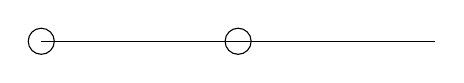
\begin{tikzpicture}
  \draw (0,0) node[circle,draw] {} -- (5,0)
  node[circle,draw,pos=0.5] {};
\end{tikzpicture}

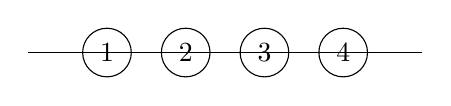
\begin{tikzpicture}
  \draw (0,0) -- (5,0)
  node foreach \x in {1,...,4} [circle,draw,pos=\x/5] {\x};
\end{tikzpicture}

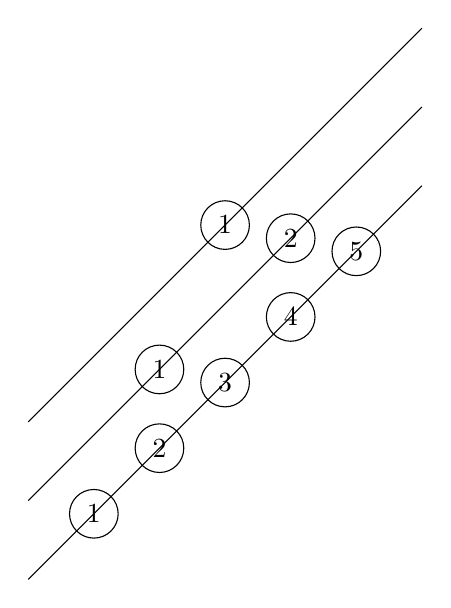
\begin{tikzpicture}
  \pic at (0,0) {tpic=5};
  \pic at (0,1) {tpic=2};
  \pic at (0,2) {tpic=1};
\end{tikzpicture}
\end{document}

%%% Local Variables:
%%% mode: latex
%%% TeX-master: t
%%% End:
